\documentclass[12pt, leqno]{article} %% use to set typesize
\input{common}

\usepackage{fontspec}
\usepackage{polyglossia}
\setmonofont{DejaVu Sans Mono}[Scale=MatchLowercase]
\usepackage[outputdir=pdf]{minted}

\providecommand{\tightlist}{%
  \setlength{\itemsep}{0pt}\setlength{\parskip}{0pt}}
\begin{document}



\hdr{2023-04-12}

\section{Life beyond Newton}

We have now seen a few iterations for solving nonlinear equations and
optimization problems from a good enough initial guess: Newton, scaled
gradient descent, and various fixed point iterations before the break;
Gauss-Newton, Levenberg-Marquardt, and IRLS at the start of this week.
Despite the variety of methods we consider, Newton's method continues to
play a central role, largely because of its rapid convergence. But while
the convergence of Newton's method is attractive, Newton steps may not
be cheap. At each step, we need to:

\begin{itemize}
\tightlist
\item
  Form the function and the Jacobian. This involves not only
  computational work, but also analytical work -- someone needs to
  figure out those derivatives!
\item
  Solve a linear system with the Jacobian. This is no easier than any
  other linear solve problem! Indeed, it may be rather expensive for
  large systems, and factorization costs cannot (in general) be
  amortized across Newton steps.
\end{itemize}

The Jacobian (or the Hessian if we are looking at optimization problems)
is the main source of difficulty. Now we consider several iterations
that deal with this difficulty in one way or the other.

\section{A running example redux}

It is always helpful to illustrate methods with an actual example. We
will continue to work with the example from before break of a nonlinear
reaction-diffusion equilibrium problem:
\[\frac{\partial v}{\partial t} = 
  \frac{\partial^2 v}{\partial x^2} + \exp(v) = 0, \quad v(0) = v(1) = 0\]
Discretizing on a mesh of points \(x_i = i/(N+1)\) with associated
function values \(v_i\), we have \[f_i(v) 
  = \frac{v_{i-1}-2v_i+v_{i+1}}{h^2} + \exp(v_i) 
  = \left[ -h^{-2} T_N v + \exp(v) \right]_i\] with \(h = (N+1)^{-1}\)
and \(v_0 = v_{N+1} = 0\). In fact, we can write
\(f(v) = -\nabla \phi(v)\) where \begin{align*}
  \phi(v) &= \frac{1}{2h^2} v^T T_N v - \sum_{i=1}^{N} \exp(v_i) \\
          &= \sum_{i=0}^n \frac{1}{2} \left( \frac{v_{i+1}-v_i}{h} \right)^2 - \sum_{i=1}^{N} \exp(v_i).
\end{align*}

\begin{minted}{julia}
function ϕ_autocatalytic(v)
    N = length(v)
    C = 0.5*(N+1)^2
    ϕ = C*v[1]^2 - exp(v[1])
    for j = 1:N-1
        ϕ += C*(v[j]-v[j+1])^2 - exp(v[j])
    end
    ϕ += C*v[N]^2 - exp(v[N])
    return ϕ
end
\end{minted}

\begin{minted}{julia}
function autocatalytic(v)
    N = length(v)
    fv        = exp.(v)
    fv        -= 2*(N+1)^2*v
    fv[1:N-1] += (N+1)^2*v[2:N  ]
    fv[2:N  ] += (N+1)^2*v[1:N-1]
    fv
end
\end{minted}

\begin{minted}{julia}
function Jautocatalytic(v)
    N = length(v)
    SymTridiagonal(exp.(v) .- 2*(N+1)^2, (N+1)^2 * ones(N-1))
end
\end{minted}

\begin{figure}
\begin{center}
  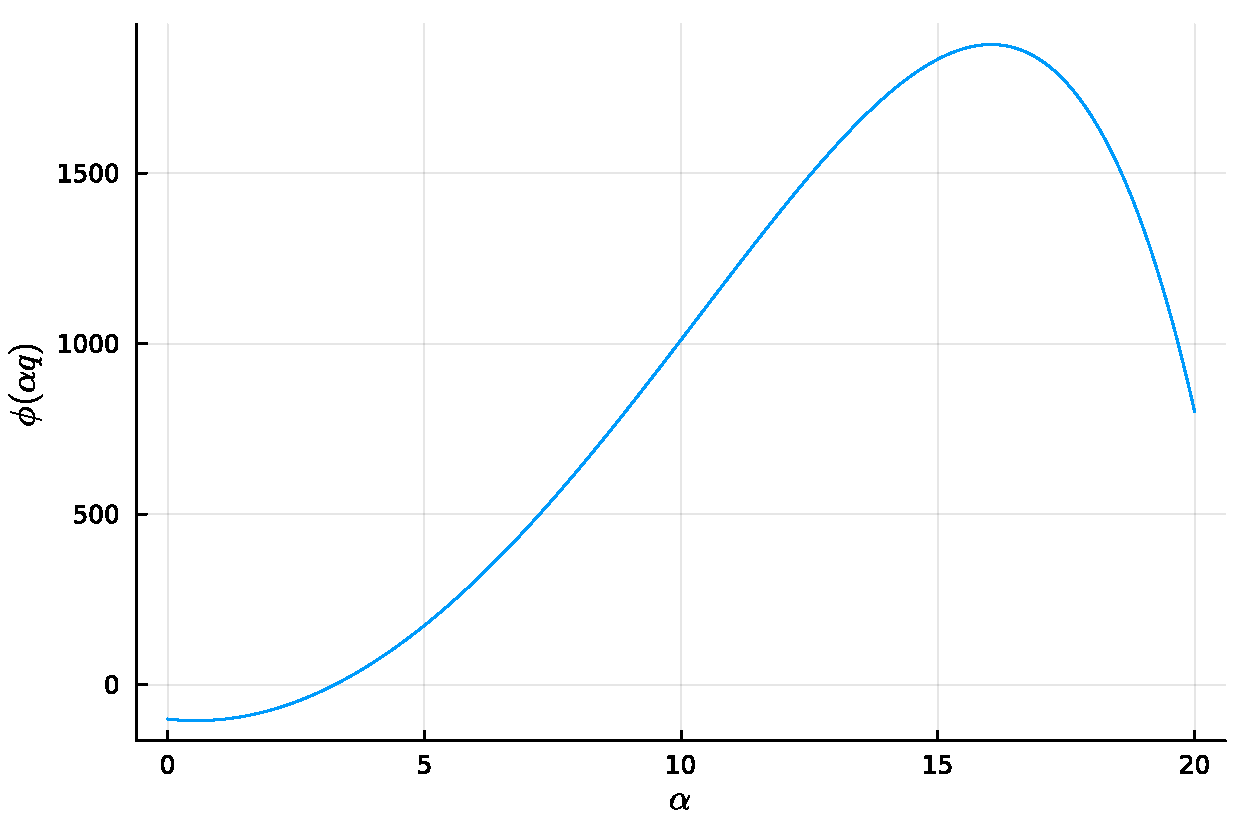
\includegraphics[width=0.8\textwidth]{fig/2023-04-12-phi-alpha.pdf}
\end{center}
\caption{Plot of energy $\phi(\alpha q)$ vs $\alpha$ for the blowup example.}
\label{fig:phi-alpha}
\end{figure}

We plot $\phi(\alpha q)$ against $\alpha$ in Figure~\ref{fig:phi-alpha}.

\begin{minted}{julia}
begin
    N = 100
    xx = range(1, N, length=N)/(N+1)
    q = xx.*(1.0 .- xx)
    plot(range(0, 20, length=1001), (α) -> ϕ_autocatalytic(α*q),
         xlabel="\$\\alpha\$", ylabel="\$\\phi(\\alpha q)\$",
         legend=false)
end
\end{minted}

\subsection{Questions}

Write a one-dimensional Newton method to find the optimal \(\alpha\) (we
will use \(\alpha = 0.5\) as an excellent starting guess throughout
these notes).

\section{Almost-Newton analysis (optional)}

In these notes, we will be somewhat careful about the analysis, but in
general you are not responsible for remembering this level of detail. We
will try to highlight the points that are important in practice for
understanding when solvers might run into trouble, and why.

A common theme in the analysis of ``almost Newton'' iterations is that
we can build on Newton convergence. We assume throughout that \(f\) is
\(C^1\) and the Jacobian is Lipschitz with constant \(M\). To simplify
life, we will also assume that \(\|f'(x)^{-1}\| \leq B\) in some
neighborhood of a desired \(x^*\) such that \(f(x^*) = 0\). Consider
what happens when we subtract the equation defining the Newton step from
a Taylor expansion with remainder of \(f(x^*)\) centered at \(x\):
\begin{align*}
  f(x) + &f'(x) p(x) = 0 \\
-[f(x) + &f'(x)(x^*-x) + R(x) = 0] \\\hline
         &f'(x)(p(x)-(x^*-x)) - R(x) = 0.
\end{align*} or \[p(x) = -(x-x^*) + f'(x)^{-1} R(x) = -(x-x^*) + d(x).\]
Under the bounded inverse hypothesis and the Lipschitz bound on \(f'\),
we know that
\[\|x + p(x) - x^*\| = \|d(x)\| \leq \frac{BM}{2} \|x-x^*\|^2\] and so
the iteration \(x \mapsto x + p(x)\) converges quadratically from
starting points near enough \(x^*\). Moreover, a sufficient condition
for convergence is that the initial error is less than \(2/(BM)\).

Now suppose we have an iteration \[x^{k+1} = x^k + \hat{p}^k\] where we
think of \(\hat{p}^k\) as an approximation to the Newton step
\(p(x^k)\). Subtracting \(x^*\) from both sides and adding
\(0 = p(x^k)-p(x^k)\) to the right hand side gives
\[e^{k+1} = e^k + p(x^k) + \hat{p}^k - p(x^k).\] Triangle inequality and
our Newton convergence result gives
\[\|e^{k+1}\| \leq \frac{BM}{2} \|e^k\|^2 + \|\hat{p}^k - p(x^k)\|.\]
Therefore, we can think of our convergence analysis in two steps: we
first analyze the error in the Newton iteration, then analyze how close
our approximate Newton step is to a true Newton step.

\section{Newton iteration}

We ran Newton iteration for the autocatalytic problem last time, but
let's run it again this time using an initial guess of \(\alpha = 0.5\).
Convergence from this initial guess is extremely rapid.

\begin{figure}
\begin{center}
  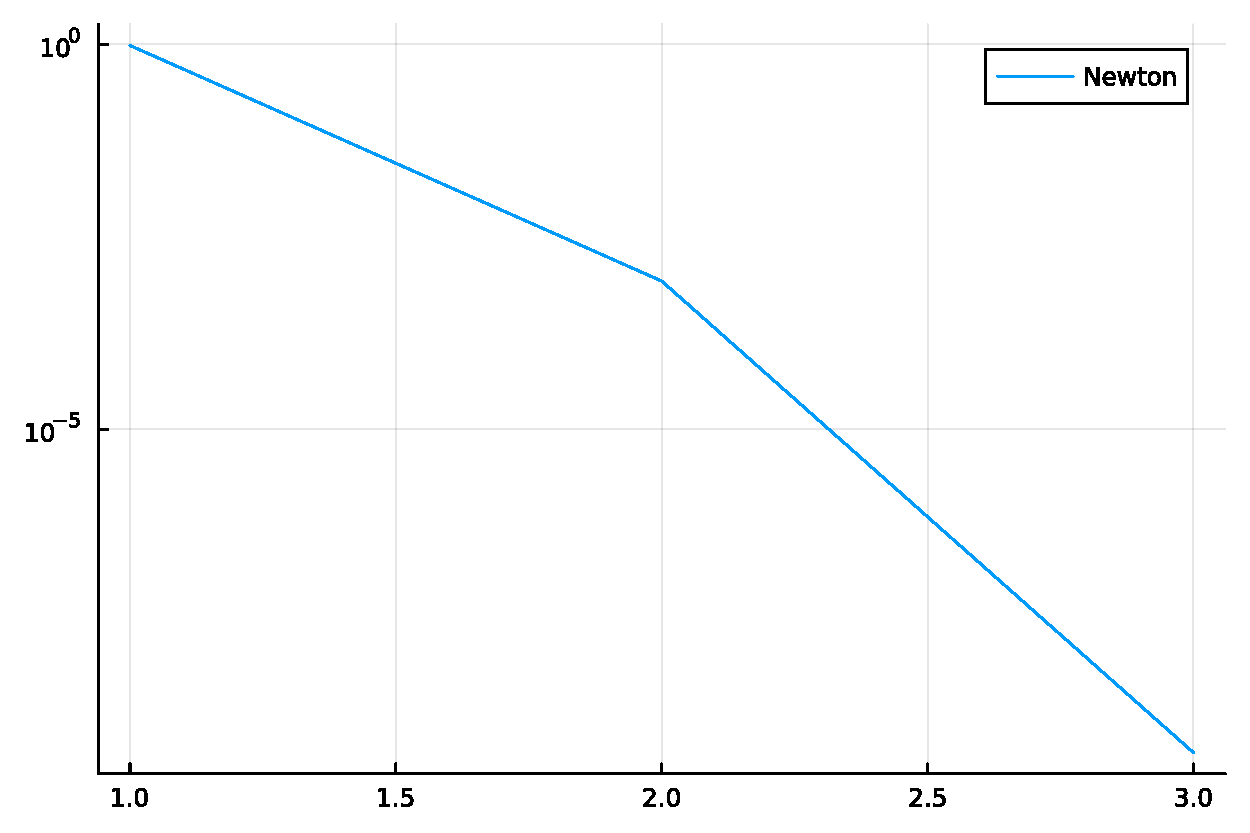
\includegraphics[width=0.8\textwidth]{fig/2023-04-12-newton.pdf}
\end{center}
\caption{Convergence of Newton for the autocatalytic blowup problem.}
\label{fig:newton-cvg}
\end{figure}

We plot convergence of Newton iteration in Figure~\ref{fig:newton-cvg}.

\begin{minted}{julia}
let
    v = 0.5*q
    rhist = []
    for k = 1:10
    	fv = autocatalytic(v)
    	v -= Jautocatalytic(v)\fv
    	push!(rhist, norm(fv))
    	if norm(fv) < 1e-9
            break
    	end
    end
    plot(rhist, yscale=:log10, label="Newton")
end
\end{minted}

\subsection{Questions}

What happens if you change the residual tolerance from \(10^{-9}\) to
\(10^{-16}\)? Why?

\section{Chord iteration}

The chord iteration is \[x^{k+1} = x^k - f'(x^0)^{-1} f(x^k)\] Written
in this way, the method differs from Newton in only one character ---
but what a difference it makes! By re-using the Jacobian at \(x^0\) for
all steps, we degrade the progress per step, but each step becomes
cheaper. In particular, we can benefit from re-using a factorization
across several steps (though this is admittedly more of an issue when
the matrix is not tridiagonal!). In terms of the approximate Newton
framework, the error behaves like \[\|e^{k+1}\| = O(\|e^0\| \|e^k\|).\]

\begin{figure}
\begin{center}
  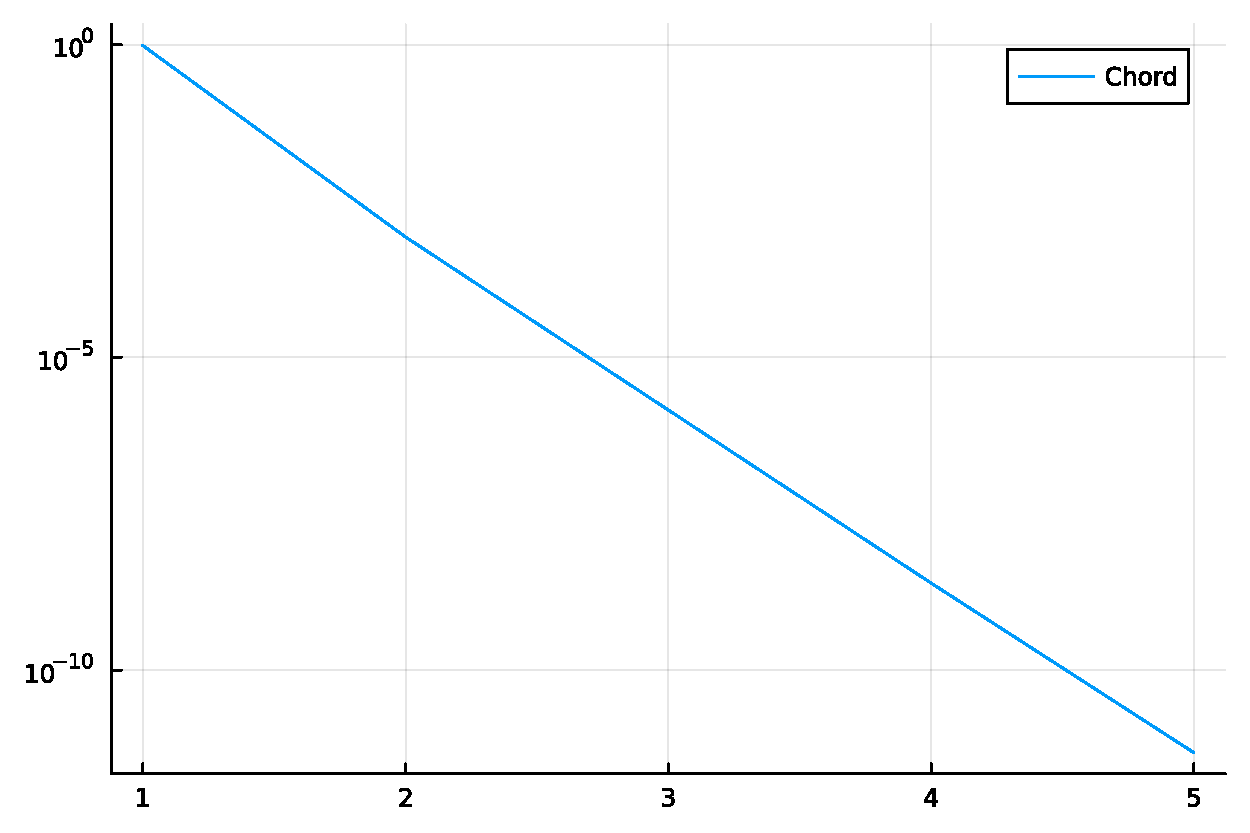
\includegraphics[width=0.8\textwidth]{fig/2023-04-12-chord.pdf}
\end{center}
\caption{Convergence of chord iteration for the autocatalytic blowup problem.}
\label{fig:chord-cvg}
\end{figure}

We plot convergence of chord iteration in Figure~\ref{fig:chord-cvg}.

\begin{minted}{julia}
let
    rhist = []
    v = 0.5*q
    J0F = ldlt(Jautocatalytic(v))  # Compute an LDL^T factorization of J
    for k = 1:10
    	fv = autocatalytic(v)
    	v -= J0F\fv
    	push!(rhist, norm(fv))
    	if norm(fv) < 1e-9
            break
    	end
    end
    plot(rhist, yscale=:log10, label="Chord")
end
\end{minted}

\subsection{Questions}

Play with \(\alpha\) in the code above to verify that the rate of
convergence depends on the quality of the initial guess.

\section{Shamanskii iteration}

The chord method involves using one approximate Jacobian forever. The
Shamanskii method involves freezing the Jacobian for \(m\) steps before
getting a new Jacobian; that is, one step of Shaminskii looks like
\begin{align*}
x^{k+1,0} &= x^k \\
x^{k+1,j+1} &= x^{k+1,j} + f'(x^k)^{-1} f(x^{k+1,j}) \\
x^{k+1} &= x^{k+1,m}.
\end{align*} Like the chord iteration, Shaminskii converges for
sufficiently close starting points, with
\[\|e^{k+1}\| = O(\|e^k\|^{m+1})\] where \(e^k\) is the error at a full
step (not one of the internal iterations).

\begin{figure}
\begin{center}
  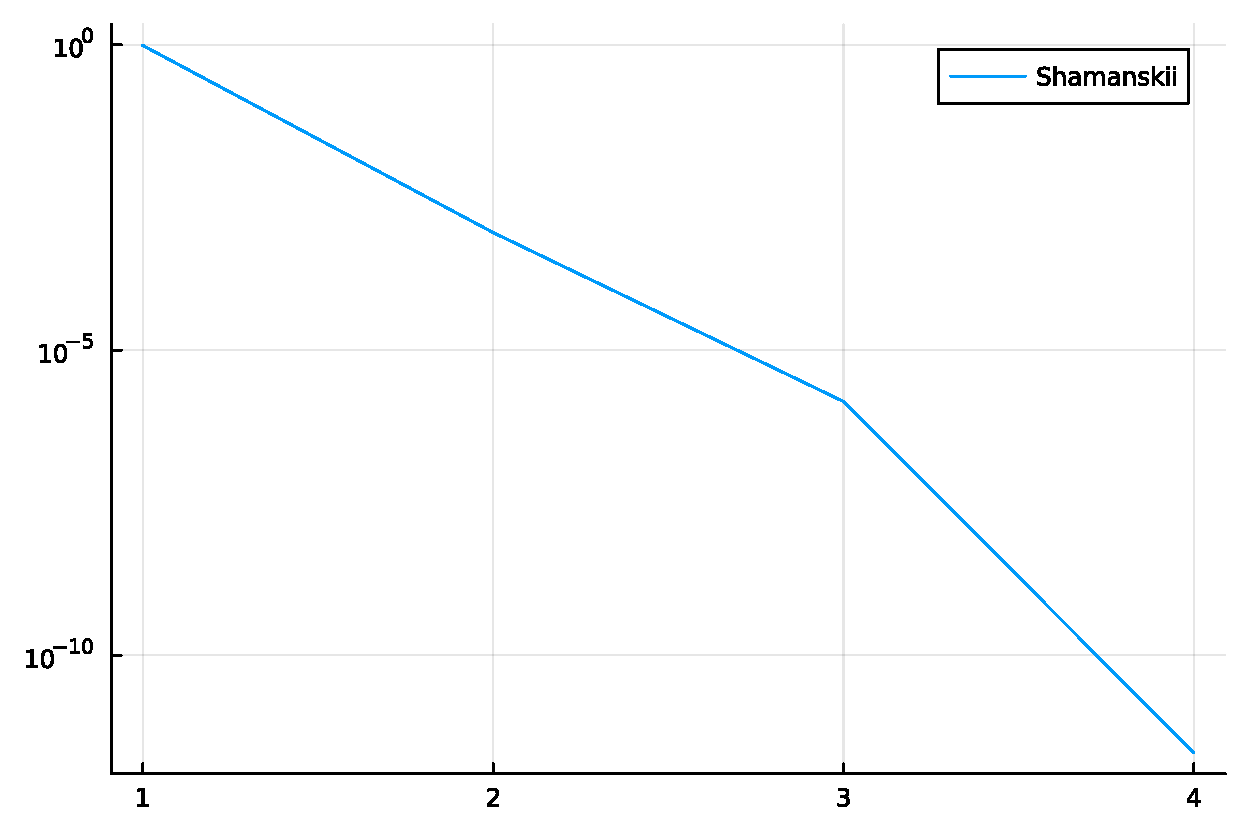
\includegraphics[width=0.8\textwidth]{fig/2023-04-12-shaminskii.pdf}
\end{center}
\caption{Convergence of Shaminskii iteration for the autocatalytic blowup problem.}
\label{fig:shaminskii-cvg}
\end{figure}

We plot convergence of Shaminskii iteration in Figure~\ref{fig:shaminskii-cvg}.

\begin{minted}{julia}
let
    m = 2
    rhist = []
    v = 0.5*q
    JF = ldlt(Jautocatalytic(v))  # Compute an LDL^T factorization of J
    for k = 1:10
    	fv = autocatalytic(v)
    	v -= JF\fv
    	push!(rhist, norm(fv))
    	if norm(fv) < 1e-9
            break
    	end
    	if mod(k, m) == 0
            JF = ldlt(Jautocatalytic(v))
    	end
    end
    plot(rhist, yscale=:log10, label="Shamanskii")
end
\end{minted}

Beyond the chord and Shaminskii iterations, the idea of re-using
Jacobians occurs in several other methods.

\section{Finite-difference Newton}

So far, we have assumed that we can compute the Jacobian if we want it.
What if we just don't want to do the calculus to compute Jacobians? A
natural idea is to approximate each column of the Jacobian by a finite
difference estimate:
\[f'(x^k) e_j \approx \frac{f(x^k+he_j)-f(x^k)}{h}.\] In general, the
more analytic information that we have about the derivatives, the better
off we are. Even knowing only the sparsity pattern of the Jacobian gives
us a lot of information. In our example, changing \(v_j\) changes
\(f_{j-1}\), \(f_j\), and \(f_{j+1}\), but not any other. Hence, we
don't actually need \(N+1\) evaluations of \(f\) to estimate the
Jacobian; we can do it with four that are cleverly chosen.

\begin{minted}{julia}
function Jtridiagonal_fd(f, x, h)
    N = length(x)

    dd = zeros(N)   # Diagonal elements
    dl = zeros(N-1) # Subdiagonal elements
    du = zeros(N-1) # Superdiagonal elements
    
    fx = f(x)
    xp = copy(x)
    for j = 1:3
        xp[:] = x
        xp[j:3:N] .+= h
        df = (f(xp)-fx)/h
        for i = 1:N
            if mod(i-j,3) == 0
                dd[i] = df[i]
            elseif mod(i-j,3) == 1 && i > 1
                dl[i-1] = df[i]
            elseif mod(i-j,3) == 2 && i < N
                du[i] = df[i]
            end
        end
    end

    return Tridiagonal(dl, dd, du)
end
\end{minted}

Convergence of Newton with a first-order finite-difference approximation
to the Jacobian is \[\|e^{k+1}\| = O(h\|e^k\|) + O(\|e^k\|^2).\]

\subsection{Questions}

Can you explain what is going on in the \texttt{Jtridiagonal\_fd} code
above?

\section{Inexact Newton}

So far, we have considered approximations to the Newton step based on
approximation of the Jacobian matrix. What if we instead used the exact
Jacobian matrix, but allowed the update linear systems to be solved
using an iterative solver? In this case, there is a small residual with
norm \(\eta_k\), and the error behaves like
\[\|e^{k+1}\| = O(\eta_k \|e^k\|) + O(\|e^k\|^2).\] Hence, we have the
following trade-off. If we solve the systems very accurately (\(\eta_k\)
small), then inexact Newton will behave much like ordinary Newton. Thus,
we expect to require few steps of the outer, nonlinear iteration; but
the inner iteration (the linear solver) may require many steps to reach
an acceptable residual tolerance. In contrast, if we choose \(\eta_k\)
to be some modest constant independent of \(k\), then we expect linear
convergence of the outer nonlinear iteration, but each step may run
relatively fast, since the linear systems are not solved to high
accuracy.

One attractive feature of Krylov subspace solvers for the Newton system
is that they only require matrix-vector multiplies with the Jacobian ---
also known as directional derivative computations. We can approximate
these directional derivaties by finite differences to get a method that
may be rather more attractive than computing a full Jacobian
approximation by finite differencing. However, it is necessary to use a
Krylov subspace method that tolerates inexact matrix vector multiplies
(e.g.~FGMRES).


\end{document}
